\chapter{The SpinTaylorF2 waveform model} 

\label{chap:SpinTaylorF2} 
The SpinTaylorF2 waveform~\cite{Lundgren2014} is a single spin, frequency
domain waveform model that incorporates the effects of precession. In the
following sections, we first define the standard notations and conventions
used to describe precessing binaries, and then discuss the construction of the
SpinTaylorF2 waveform model.

\section{Notations and conventions}
Consider a NSBH binary, with black hole mass $m_{1}$ and dimensionless spin
$\chi_{1} = |\mathbf{S}|/m_{1}^2$ where $|\mathbf{S}|$ is the spin angular
momentum of the black hole, and a neutron star with mass $m_{2}$ and zero
spin. The the symmetric mass ratio $\eta$ is defined as $\eta=m_{1}m_{2}/M^2$,
where $M$ corresponds to the total mass of the binary $(m_{1} + m_{2})$.
Further, we can define the total angular momentum vector
$\mathbf{J}=\mathbf{L} + \mathbf{S}$ of the binary as the sum of the orbital
angular momentum vector $\mathbf{L}$. We also define the spin-alignment parameter
$\kappa=\hat{\mathbf{L}}\cdot\hat{\mathbf{S}}$, to describe the alignment of
the $\mathbf{L}$ and $\mathbf{S}$: $\kappa=0$ corresponds to the situation
where $\mathbf{L}$ and $\mathbf{S}$ are perpendicular to each other, and
$\kappa=\pm 1$ corresponds to the aligned (anti-aligned) case. In addition,
polar angles $(\theta_{J}, \psi_{J})$  describes the relative orientation  of
the total angular momentum vector $\mathbf{J}$ with the line of sight unit
vector $\hat{\mathbf{N}}$ (see, for eg.,~\cite{thetaJ} for a graphical
representation of the coordinates used). All the equations in the report are
written in $\left[G = c = M_{\odot }= 1\right]$ units.

\section{Inertial and co-rotating frames of reference}


\begin{figure}[t]
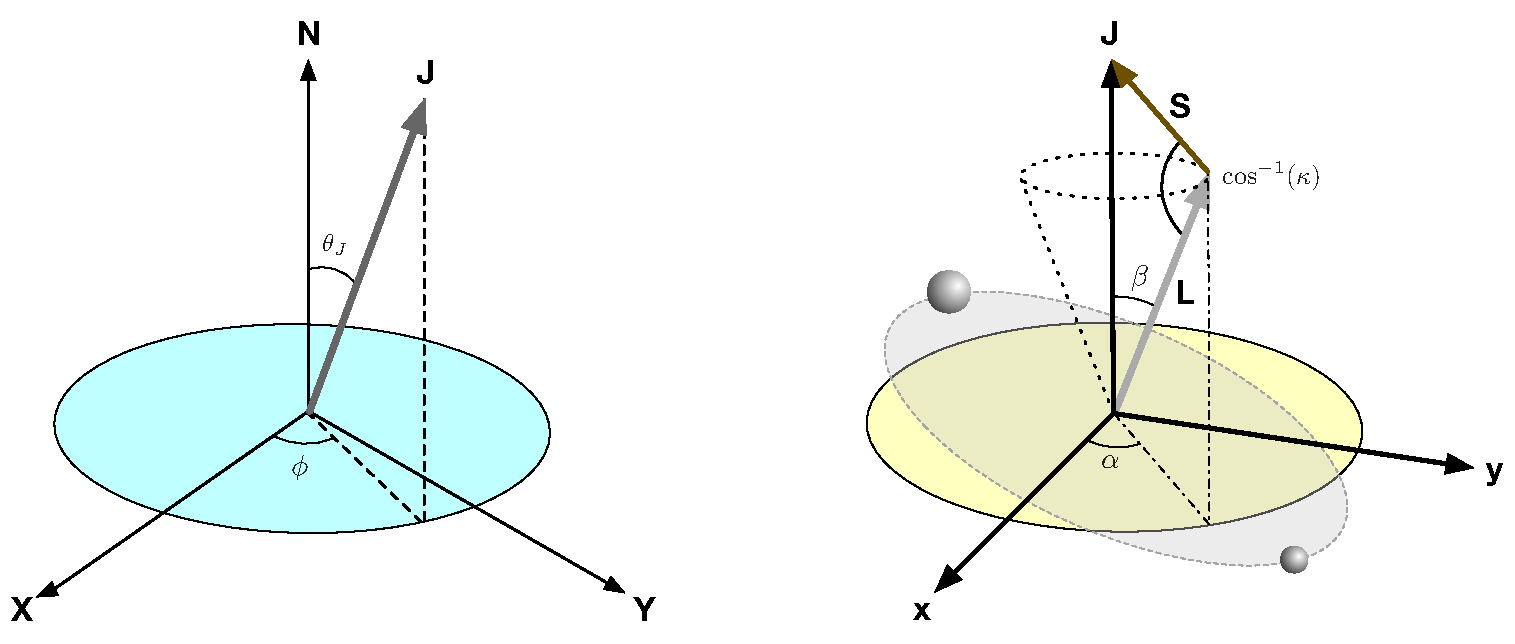
\includegraphics[width=0.8\textwidth]{./images/STF2_coordinates.pdf}
\centering 
\caption{Detector (left) and inertial frame (right) of reference for
precessing systems.}
\centering 
\label{fig:frames} 
\end{figure}

If the black hole has non-zero spin, and the spin-angular momentum
$\mathbf{S}$ is  not aligned with the orbital orbital angular momentum
$\mathbf{L}$ of the binary, the plane of orbital motion inclines and precesses
over time~\cite{Apostolatos1994}. Concretely, both $\mathbf{L}$ and
$\mathbf{S}$  would precess about the total angular momentum vector
$\mathbf{J}$. Further, if one of the components of the binary has zero spin,
the binary undergoes simple precession. In such a case, the time evolution of  
$\mathbf{L}$ and $\mathbf{S}$ is given by:

\begin{dgroup}
\begin{dmath}
\dot{L} = \dfrac{-32}{5} \dfrac{{\mu}^2}{r} \left(\dfrac{M}{r}\right)^{5/2}
\end{dmath}
\begin{dmath}
\dot{S} = 0
\end{dmath}
\begin{dmath}
\dot{\hat{\textbf{L}}} = \left(2 + \dfrac{3 m_2}{2 m_1} \right)
\dfrac{\textbf{J}}{r^3} \times \hat{\textbf{L}}
\end{dmath}
\begin{dmath}
\dot{\hat{\textbf{S}}} = \left(2 + \dfrac{3 m_2}{2 m_1} \right)
\dfrac{\textbf{J}}{r^3} \times \hat{\textbf{S}}
\end{dmath}
\end{dgroup}

where $\mu$ is the reduced mass of the binary. Since the angle between
$\mathbf{L}$ and $\mathbf{S}$ do not change over precession cycles, we define
two additional ratios

\begin{equation}
\gamma \equiv \dfrac{|\textbf{S}_1|}{|\textbf{L}|} = \dfrac{m_1 \chi}{m_2} v
\end{equation}
\begin{equation}
\Gamma_J \equiv \dfrac{|\textbf{J}|}{|\textbf{L}|} = \sqrt{1 + 2 \kappa \gamma + {\gamma}^2}
\end{equation}

In the simple precession approximation, $\mathbf{J}$ remains nearly fixed
during the inspiral, and $\mathbf{L}$ and $\mathbf{S}$ precesses about
$\mathbf{J}$ with a uniform angular velocity $\Omega_{\rm p} = \eta (2 + 3
m_2/2m_1)\,v^4 \,\Gamma_J$ and the opening angle of the precession code is
equal to $\beta = \cos^{-1}\left[(1 +
\kappa\gamma)/\Gamma_J\right]$. The SpinTaylorF2 waveform assumes simple
precession~\cite{Lundgren2014}, and breaks down when the assumption is no
longer applicable.

To describe the dynamics of the system, therefore, we introduce two different
frames of reference. The first frame (called the inertial or observer's frame
of reference) is aligned with the total angular momentum vector $\mathbf{J}$,
and, therefore fixed in space. The other frame co-rotates with the orbital
plane, i.e., is always instantaneously aligned with the direction of the
orbital angular momentum, and is therefore referred to as the non-inertial
(co-rotating) frame of reference. See Fig.~\ref{fig:frames}, which shows the
orientation of $\mathbf{J}$ and $\mathbf{L}$ with the detector frame (left)
and inertial frame (right), respectively. 


\begin{figure}[t]
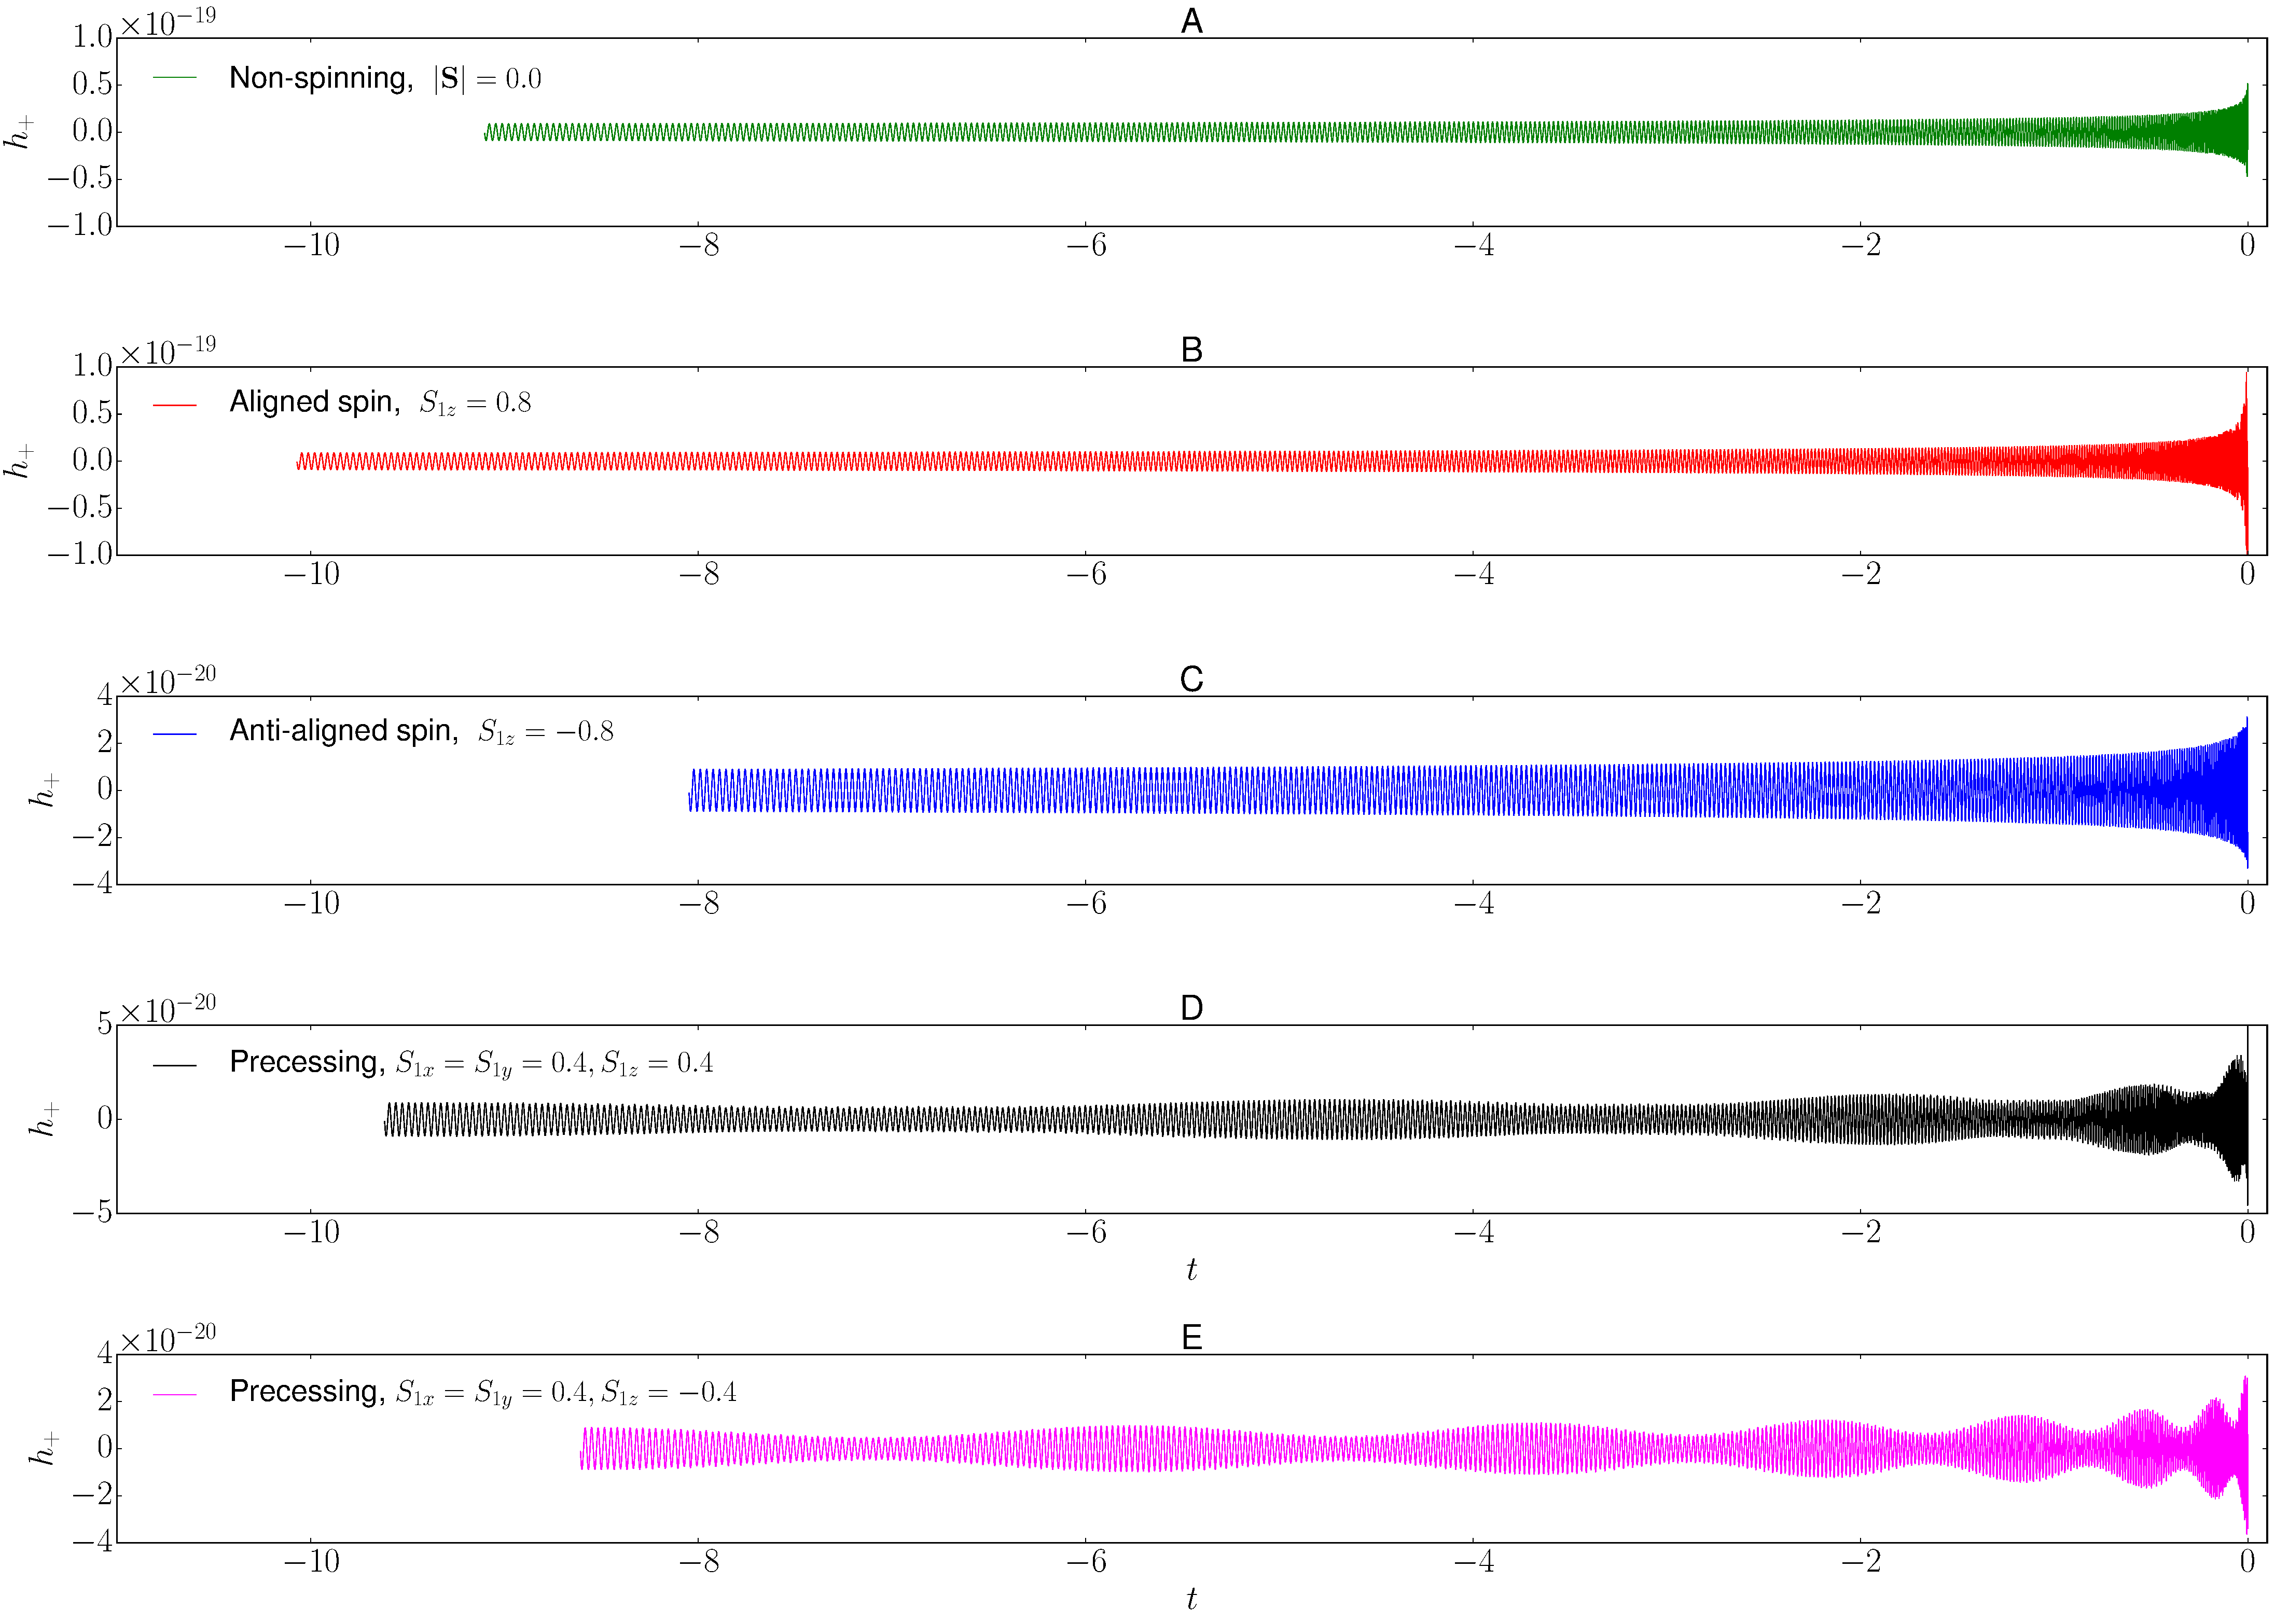
\includegraphics[width=\textwidth]{./images/SPT2_waveforms.pdf}
\caption{SpinTaylorT2 waveforms for non-precessing (A, B, C) and precessing
(D, E) systems.}
\centering 
\label{fig:waveforms} 
\end{figure}

The precession of the orbital plane leads to modulations in the gravitational
wave amplitude and phase in the observer's frame of reference.
Fig.~\ref{fig:waveforms} shows the effects of precession on the gravitational
waveform, generated using the SpinTaylorT2 waveform model~\cite{STT2}. The
first three panels (A, B and C) show non-precessing waveforms with zero spin,
and aligned and anti-aligned values of $\kappa$. The last two panels
correspond to waveforms from a precessing system and are for a generic
orientation of spin. These waveforms are modulated both in amplitude and
phase, because of the precession of $\mathbf{L}$ and $\mathbf{S}_1$ about
$\mathbf{J}$. From the figure, the effect of precession on waveform amplitude
is evident. In addition to the inspiral time scale, the precession introduces
a new time scale which is responsible for the waveform modulation. Further,
the rate of precession also changes during the inspiral phase (depending on
the spin alignment parameter $\kappa$), which in turn introduces
characteristic variations in the modulations of the waveform.


\section{The construction of SpinTaylorF2}

The construction of the waveform model is based on the assumption that a
precessing waveform in the inertial frame of reference can be
\textit{approximately mapped} into a non-precessing waveform acted upon by a
time-dependent rotation~\cite{Schmidt2012,Boyle2011, Rotation}. The 
time-dependent rotation relates the inertial frame of reference aligned with
$\mathbf{J}$ to the source (non-inertial) frame that co-rotates with the orbital
angular momentum vector $\mathbf{L}$. The precessing waveform can then be
expressed as a weighted sum of the co-rotating frame amplitudes
$\tilde{h}^{l,m}$ (see Eq. (3) in~\cite{Lundgren2014}):
\begin{equation}   
h_{+}(t) + i h_{\times}(t) = e^{-2 \psi(t)}
\sum_{l,m,m^{\prime}} \mathcal{D}^{l}_{m^{\prime},m} \left(\alpha(t), \beta(t), \gamma(t)\right)
\tilde{h}^{l,m}(t){}_{-2}Y_{l,m^{\prime}}\left(\theta,\phi\right)e^{-i m \Phi(t)},
\end{equation}   
where $\mathcal{D}^{l}_{m^{\prime},m}$ is the Wigner rotation matrix of
SU2~\cite{Boyle2011}, and $(\alpha(t), \beta(t), \gamma(t))$ are the time-
dependent Euler angles that relate the co-rotating frame to the inertial frame
of reference, and $\Phi(t)$ corresponds orbital phase of the waveform.
Considering only the leading order $(l=2, |m| = 2)$ mode, we can express the
above expression in frequency domain using the Stationary Phase
Approximation~\cite{Lundgren2014, Creighton}. In the case of simple
precession, the precession time scale is much smaller than the inspiral time
scale, and therefore, $\beta$ is considered to be a constant over several
precession cycles. Further, the assumption that the orbital phase is
independent of $\alpha$ and $\zeta$ ensures that the
precession-induced phase varies much slowly than the orbital phase, which
allows for the use of stationary phase approximation to obtain the closed-form
expression for the waveform in the frequency domain. Upon simplification, one
arrives at the following frequency domain expression for the SpinTaylorF2
waveform (see Eq. (12 --13) in~\cite{Lundgren2014}):
\begin{equation}  
\label{STF2_main} 
h_{+}(f) =
\dfrac{2\pi M_{c}^{2}}{D}\sqrt{\dfrac{5}{96\pi}}(\pi M
f)^{-7/6}\sum_{m}z_{m}e^{i(\Psi(f) - 2\zeta(f)) + i m \alpha(f)},
\end{equation} 
where $D$ corresponds to the distance to the source, $M_{c}=(m_1 m_2)^(3/5)/(m_1 +
m_2)^{1/5}$ corresponds to chirp mass of the binary, $\Psi(f) = 2 \pi f t(f) -
2 \Phi(t(f))$, and $\alpha(f)$ and $\zeta(f)$ are related to
\begin{eqnarray}
\alpha(v) &=& \eta \left( 2 + \dfrac{3 m_2}{2 m_1}\right) \int v^5 \Gamma_J \dfrac{dt}{dv}dv, \\
\zeta(v) &=& \eta \left( 2 + \dfrac{3 m_2}{2 m_1}\right) \int v^5 (1 + \kappa\gamma) \dfrac{dt}{dv}dv,
\end{eqnarray}
using the relation between orbital velocity and orbital frequency, given by $v = (M
\omega)^{(1/3)}$. Further, $z_{m}$'s are normalized amplitude functions, which
when expressed in terms of the spin-weighted spherical harmonics read
\begin{equation}\label{zm}
z_m(\theta_J, \psi_J, \beta(f)) = \frac{4\pi}{5} \, \mathstrut_{-2}Y_{2,m}(\beta(f), 0)
\left[  e^{-2i\psi_J} \;  \mathstrut_{-2}Y_{2,m}(\theta_J,0) 
+ e^{2i\psi_J}  \; \mathstrut_{-2} Y_{2,-m}(\theta_J,0) \right].
\end{equation}
Each term in the summation (labeled by $m$) in Eq.~(\ref{STF2_main})
represents a single sideband that is modulated in amplitude and phase
depending on the value of $m$. One can show, using the analytical expressions
for $z_m$, that only $m=2$ sideband has a non-zero amplitude when the system
is non-precessing $(\beta=0)$; however, for a precessing system, all the
sidebands develop a non-zero amplitude. The factor of $z_m$ therefore, is
responsible for introducing amplitude modulations to the waveform, and is also
dependent on the orientation of the binary.





